% Generated by make_thesis_pgfplots.py -- do not edit by hand.
\definecolor{vizblue}{HTML}{2A78D6}
\definecolor{vizorange}{HTML}{EB6834}
\definecolor{vizgrid}{HTML}{E1E0D9}
\definecolor{vizaxis}{HTML}{C3C2B7}
\definecolor{vizmuted}{HTML}{898781}
\definecolor{vizink}{HTML}{52514E}

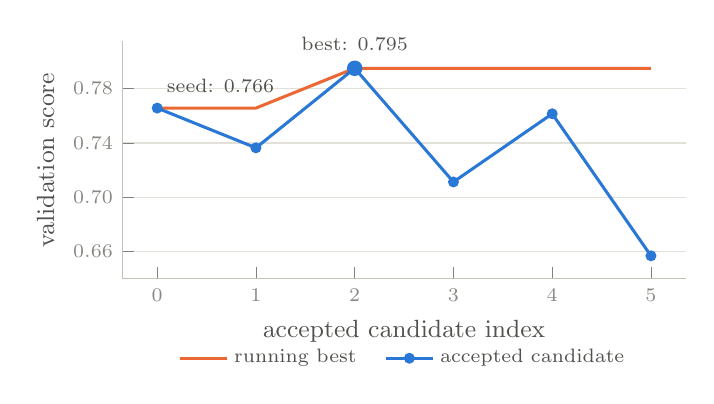
\begin{tikzpicture}
    \begin{axis}[
        width=0.72\linewidth, height=4.6cm,
        xmin=-0.35, xmax=5.35, ymin=0.64, ymax=0.815,
        xtick={0,1,2,3,4,5},
        ytick={0.66,0.70,0.74,0.78},
        yticklabel style={/pgf/number format/fixed, /pgf/number format/fixed zerofill, /pgf/number format/precision=2},
        xlabel={accepted candidate index},
        ylabel={validation score},
        legend columns=2,
        legend style={at={(0.5,-0.26)}, anchor=north, /tikz/every even column/.append style={column sep=8pt}},
        axis line style={vizaxis, line width=0.4pt},
        tick label style={vizmuted, font=\scriptsize},
        label style={vizink, font=\small},
        legend style={draw=none, fill=none, font=\scriptsize,
                      text=vizink, inner sep=1pt},
        grid=major,
        grid style={vizgrid, line width=0.4pt},
        axis x line*=bottom,
        axis y line*=left,
        ymajorgrids=true,
        xmajorgrids=false,
        clip=false,
    ]
    \addplot[vizorange, line width=1.1pt] coordinates {(0,0.7657) (1,0.7657) (2,0.7950) (3,0.7950) (4,0.7950) (5,0.7950)};
    \addlegendentry{running best}
    \addplot[vizblue, line width=1.1pt, mark=*, mark size=1.4pt, mark options={fill=vizblue, draw=vizblue}] coordinates {(0,0.7657) (1,0.7364) (2,0.7950) (3,0.7113) (4,0.7615) (5,0.6569)};
    \addlegendentry{accepted candidate}
    \addplot[only marks, mark=*, mark size=2.6pt, vizblue, forget plot] coordinates {(2,0.7950)};
    \node[anchor=south, font=\scriptsize, text=vizink] at (axis cs:2,0.8010) {best: 0.795};
    \node[anchor=south west, font=\scriptsize, text=vizink] at (axis cs:0,0.7697) {seed: 0.766};
    \end{axis}
\end{tikzpicture}
